\documentclass{article}
\usepackage{eecstex}

\title{EECS 151 HW 02}
\author{Bryan Ngo}
\date{2022-02-06}

\begin{document}

\maketitle

\section{Moment of Truth Table}

\subsection{}

\begin{tabular}{||c|c|c||c||}
    \hline
    \(A\) & \(B\) & \(C\) & \(Y\) \\
    \hline
    0 & 0 & 0 & 1 \\
    0 & 0 & 1 & 0 \\
    0 & 1 & 0 & 1 \\
    0 & 1 & 1 & 1 \\
    1 & 0 & 0 & 1 \\
    1 & 0 & 1 & 0 \\
    1 & 1 & 0 & 1 \\
    1 & 1 & 1 & 1 \\
    \hline
\end{tabular}

\subsection{}

\begin{tabular}{||c|c|c||c||}
    \hline
    \(A\) & \(B\) & \(C\) & \(Y\) \\
    \hline
    0 & 0 & 0 & 1 \\
    0 & 0 & 1 & 1 \\
    0 & 1 & 0 & 0 \\
    0 & 1 & 1 & 0 \\
    1 & 0 & 0 & 1 \\
    1 & 0 & 1 & 0 \\
    1 & 1 & 0 & 0 \\
    1 & 1 & 1 & 1 \\
    \hline
\end{tabular}

\subsection{}

\begin{tabular}{||c|c|c||c||}
    \hline
    \(A\) & \(B\) & \(C\) & \(Y\) \\
    \hline
    0 & 0 & 0 & 1 \\
    0 & 0 & 1 & 1 \\
    0 & 1 & 0 & 1 \\
    0 & 1 & 1 & 0 \\
    1 & 0 & 0 & 1 \\
    1 & 0 & 1 & 1 \\
    1 & 1 & 0 & 1 \\
    1 & 1 & 1 & 1 \\
    \hline
\end{tabular}

\newpage
\section{Boo\ldots lean}

\begin{align}
    Y &= \overline{DC + \overline{(\overline{DC} + B\overline{A}) D}} + B (\overline{A + \overline{C}}) \\
    &= (\overline{D} + \overline{C}) \cdot (\overline{\overline{(\overline{DC} + B\overline{A}) D}}) + B (\overline{A} \cdot \overline{\overline{C}}) \\
    &= (\overline{D} + \overline{C}) \cdot (\overline{DC} + B\overline{A}) D + B \overline{A} C \\
    &= (\overline{D} + \overline{C}) \cdot (\overline{D} + \overline{C} + B \overline{A}) D + B \overline{A} C \\
    &= (\overline{D} + \overline{C} + B\overline{A}) D \overline{D} +(\overline{D} + \overline{C} + B\overline{A}) D \overline{C} + B \overline{A} \cdot C \\
    &= (\overline{D} + \overline{C} + B \overline{A}) D \overline{C} + B \overline{A} C \\
    &= \overline{D} D \overline{C} + \overline{C} D \overline{C} + B \overline{A} D \overline{C} + B \overline{A} C \\
    &= D \overline{C} + B \overline{A} D \overline{C} + B \overline{A} C \\
    &= D \overline{C} + B \overline{A} (D \overline{C} + C) \\
    &= D \overline{C} + B \overline{A} C
\end{align}

\newpage
\section{K for Karnaugh Map}

\subsection{}

\begin{equation}
    \begin{pmatrix}
        0 & 0 & 0 & 0 \\
        1 & 0 & 0 & 0 \\
        1 & 1 & 0 & 0 \\
        0 & 0 & 0 & 0
    \end{pmatrix}
    \implies F = BC'D' + ABC'
\end{equation}

\subsection{}

\begin{equation}
    \begin{pmatrix}
        1 & 1 & 1 & 1 \\
        1 & 1 & 1 & 1 \\
        1 & 1 & 0 & 1 \\
        1 & 1 & 0 & 1
    \end{pmatrix}
    \implies F = A' + C' + D'
\end{equation}

\subsection{}

\begin{equation}
    \begin{pmatrix}
        0 & 1 & 0 & 0 \\
        0 & 1 & 1 & 1 \\
        0 & 1 & 0 & 0 \\
        0 & 1 & 0 & 0
    \end{pmatrix}
    \implies F = C'D + A'BD + A'BC
\end{equation}

\newpage
\section{Mealy or Moore}

This is a Mealy machine.
Converting to a Moore machine,
\begin{center}
    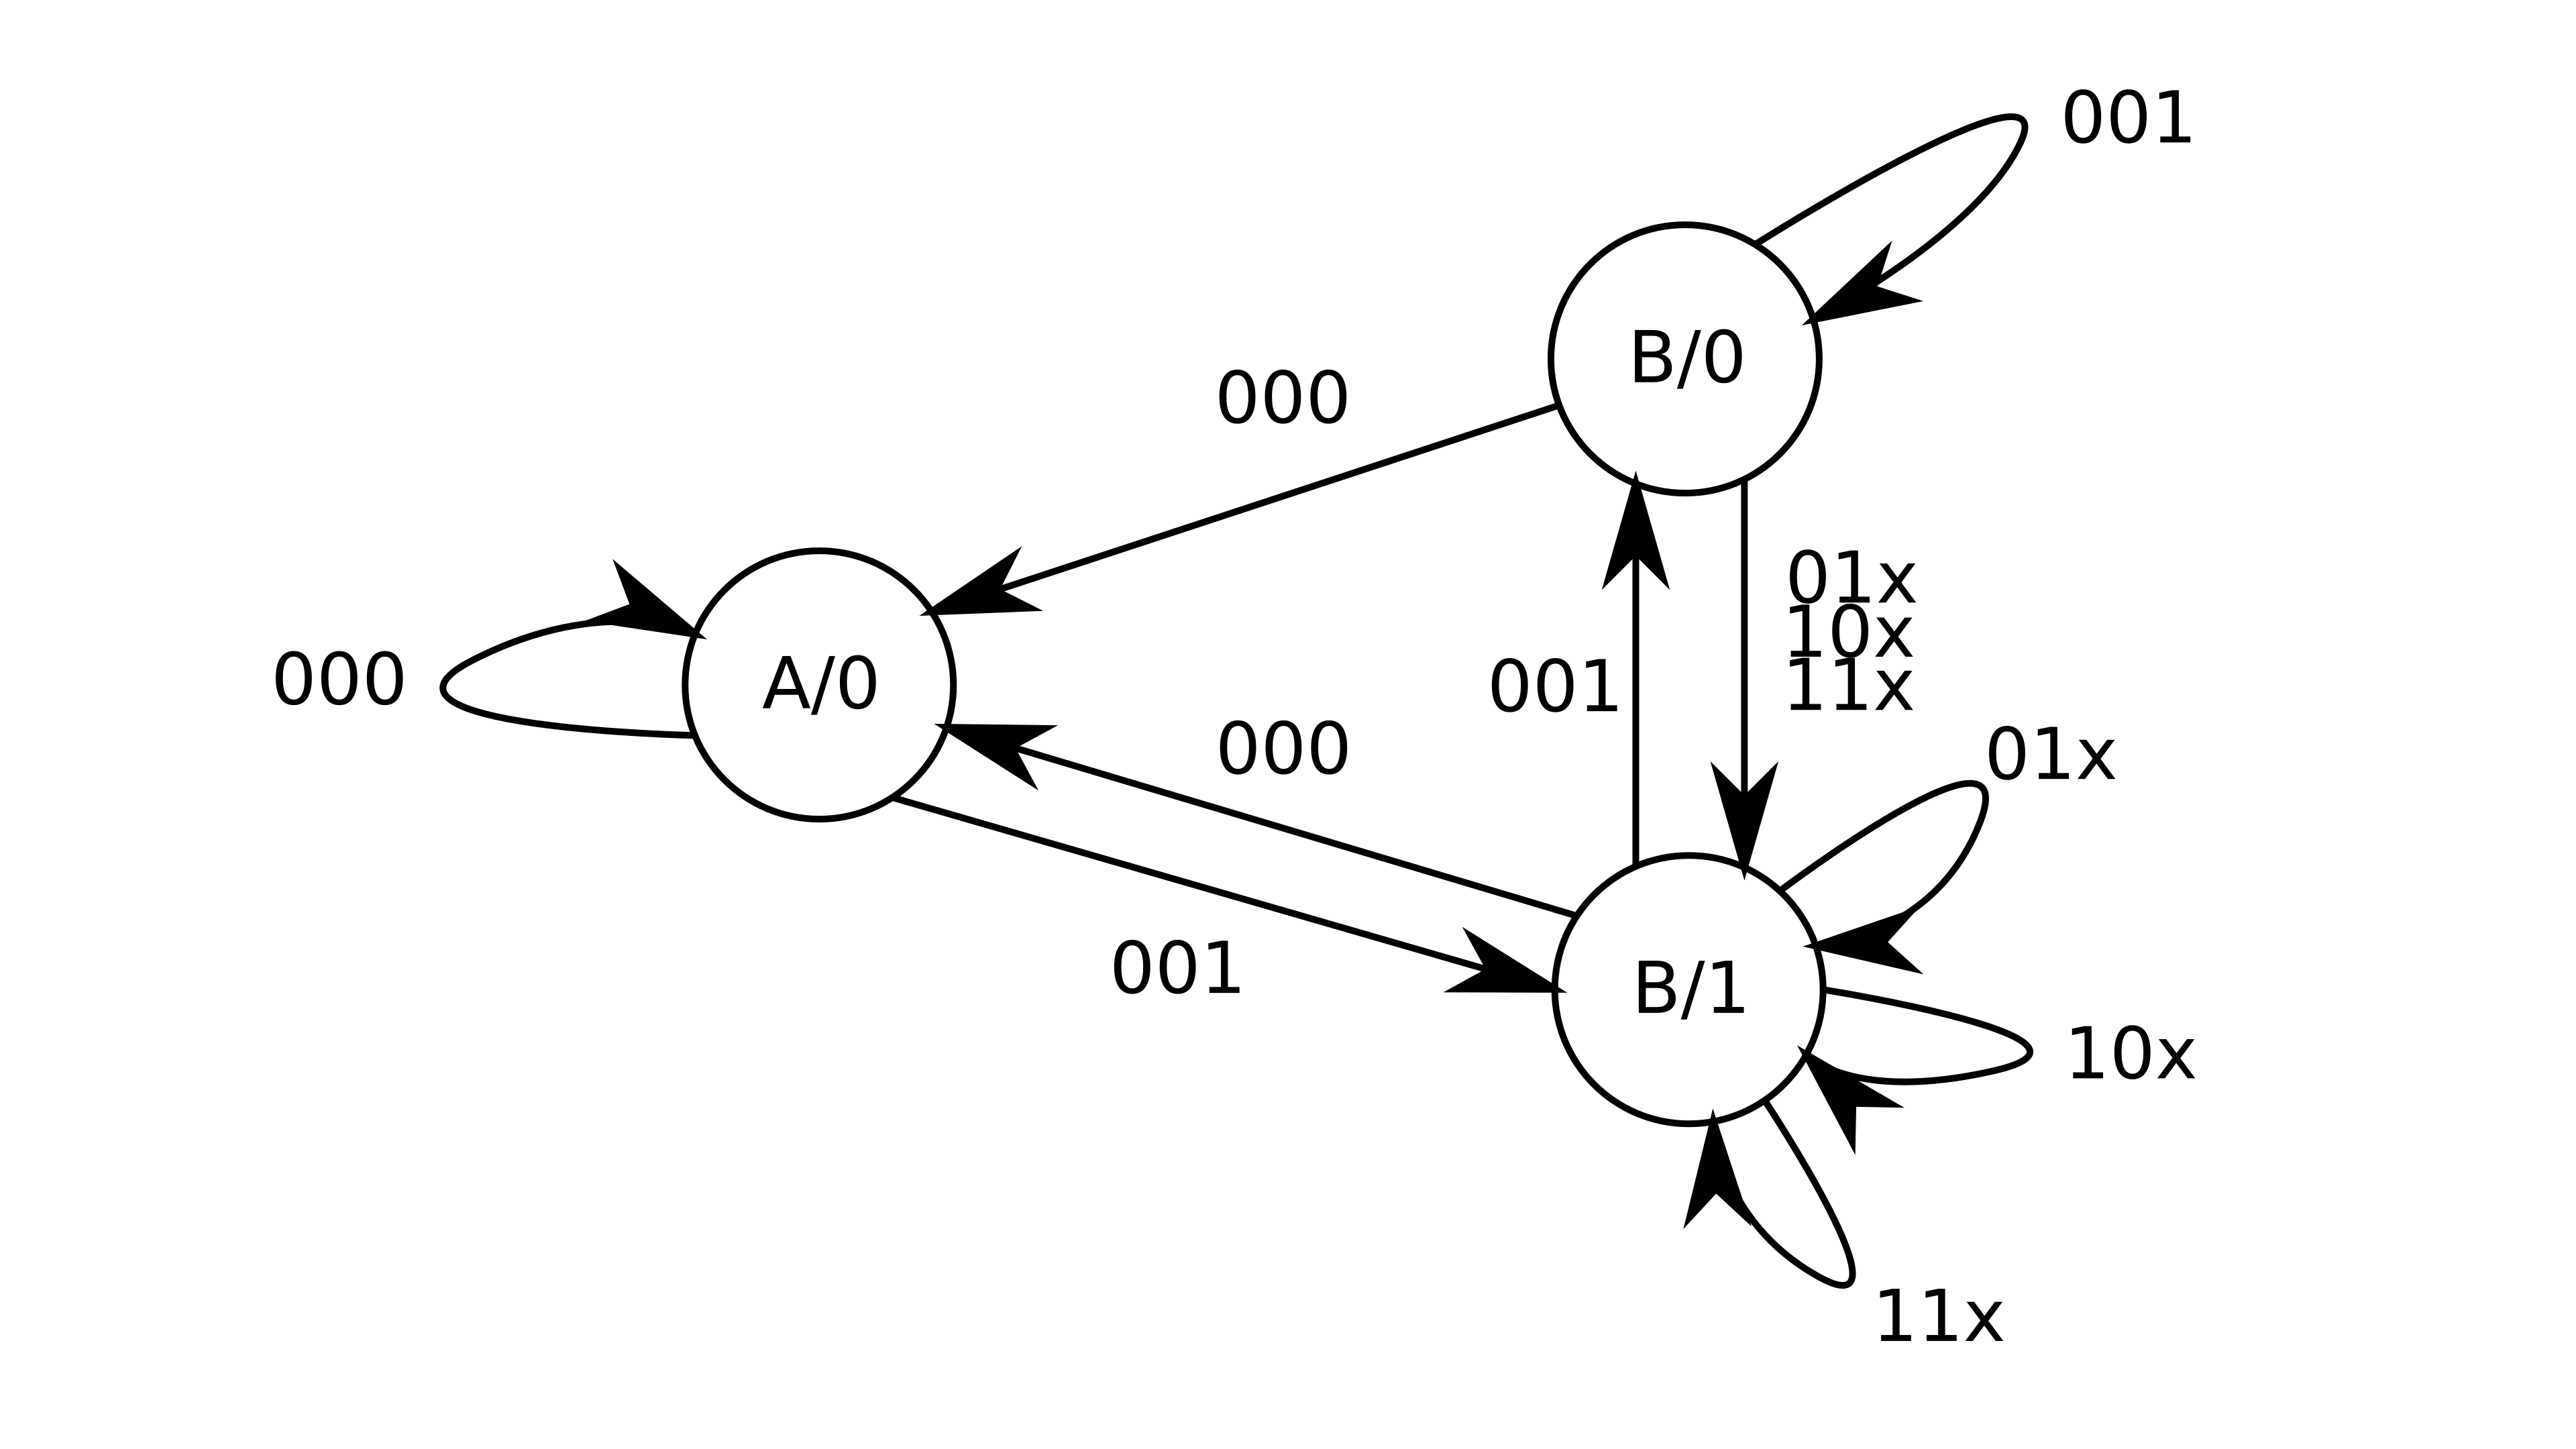
\includegraphics[width=0.6\textwidth]{q4.png}
\end{center}

\end{document}
